\documentclass[conference]{IEEEtran}
\IEEEoverridecommandlockouts
% The preceding line is only needed to identify funding in the first footnote. If that is unneeded, please comment it out.
\usepackage{cite}
\usepackage{amsmath,amssymb,amsfonts}
\usepackage{algorithmic}
\usepackage{graphicx}
\usepackage{textcomp}
\usepackage{xcolor}
\usepackage{hyperref}

% For tables
\usepackage{booktabs}
\usepackage{tabularx}
\usepackage{stfloats}
\usepackage[table]{xcolor}
\definecolor{lightgray}{gray}{0.95}



\usepackage{fancyhdr}
\pagestyle{fancy}
\lhead{Michigan Robotic Submarine}
\rhead{\thepage}

\def\BibTeX{{\rm B\kern-.05em{\sc i\kern-.025em b}\kern-.08em
    T\kern-.1667em\lower.7ex\hbox{E}\kern-.125emX}}

\usepackage{titlesec}
\titlespacing*{\subsection}{0pt}{1em}{0.3em}
\titlespacing*{\subsubsection}{0pt}{1em}{0.3em}
% 1em vertical spacing before each subsubsection and 0.5em after each subsubsection

\newcolumntype{L}{>{\raggedright\arraybackslash}X} % This column type allows the text in the table with "Component Specifications" to be left aligned (as opposed to full justification)

\begin{document}

\title{Michigan Robotic Submarine: Strategy, Design, and Implementation of Montemayor}
\author{
Zayn Baig, Muskaan Mittal, Carter Kassin, Brady Messock, Luke VanderHeuvel % Team leads
\\ 
Kaden Chirco, Thales Protopapas, Miles Pilgeram, Ashley McPike, Arnav Mummineni % Other members
}

%
% NOTE: While editing this document please reference the rubric RoboNation will be gradiing us on. We want to ensure that our sections align with that: https://robonation.gitbook.io/robosub-resources/section-2-design-documentation/2.1-technical-design-report
%

\maketitle
\pagestyle{fancy}
\lhead{Michigan Robotic Submarine}
\rhead{\thepage}

\begin{abstract}
Michigan Robotic Submarine is an undergraduate student project team at the University of Michigan in its sixth year participating in the RoboSub competition. We developed our autonomous underwater vehicle (AUV), Montemayor, shown in Fig. 1, to improve our accuracy and reliability on previous tasks while maintaining potential for future developments. To improve iteration speed, we developed a software simulator to provide software members a testing ground before running in-water verification. To enhance organization and robustness, we overhauled our motor controller PCB and developed a battery voltage monitor. To modernize our software stack, we migrated from Robot Operating System (ROS) version 1 to ROS version 2 while continuing to individualize our implementation with custom motor controller software, a custom PID controller, and a revamped machine learning stack. Finally, we laid the groundwork for future improvement like improved localization and control using our DVL, additional mechanisms to complete new tasks, and adding electrical safety mechanisms to prevent future damage and setbacks.


\end{abstract}

\section{Competition Strategy} \label{sec:comp_strat}
Competition strategy begins with aligning our robot's current and near-term planned capabilities with the highest value tasks available given those capabilities. We are continuing to use the hull we first designed in 2023, though this will our last year doing so. As such, we catered our design towards maximizing the competitive potential of our current submarine by improving AUV capabilities and system robustness. Some areas that we identified as established strengths include our machine learning pipeline, which we were able to quickly train and utilize at previous competitions, and our task planner which coordinates high-level, logical transitions between robot actions as well as mapping out failure cases and fallback states for each task. To make our system electrically robust and better organize our Electronic Speed Controllers (ESCs), we developed custom motor controller PCBs. To refine AUV capabilities, we developed a custom PID controller, custom motor controller code, and custom teleoperation code to enhance flexibility and reduce unnecessary reliance on external packages. We also migrated our software stack to ROS 2 \cite{b6} after ROS 1 reached end-of-life in June 2025.

\subsection{Target Tasks} \label{ssec:target_goals}
Our target tasks for the 2026 RoboSub competition are the Heading Out (coin flip), Begin Assessment (gate), Avoid Debris (slalom), and Return Home tasks, with a stretch goal of the Recon (bins) task.

\subsubsection{Heading Out---Coin Flip}
\label{sssec:coin_flip_task}
To complete the coin flip task, our design requires the AUV to sense its gyroscopic orientation prior to rotating according to the coin flip and starting its run. This provides a reliable method for identifying the initial angle needed to turn to face the gate, regardless of the result of the coin flip. 


\subsubsection{Begin Assessment---Gate}
\label{sssec:gate_task}
To pass through the gate, we use a machine learning model to detect the image on the gate and center on it. We decided to always choose the same image to center on, as this allows us to focus on optimizing the model’s performance for that specific image. Additionally, this makes it so that we can complete the bin and slalom tasks in the same way every run to maximize points (namely, the same side of the slalom poles and the same side target on the bin), enabling greater run-to-run consistency.

\begin{figure}
    \centerline{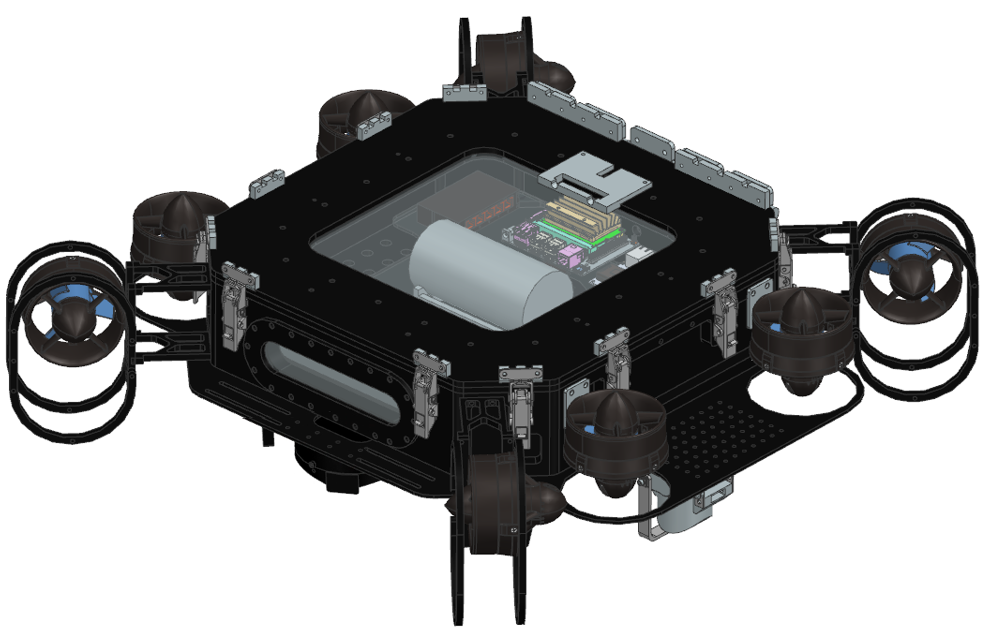
\includegraphics[scale=0.35]{images/FullSub2025-5.png}}
    \caption{CAD of our 2025-2026 AUV, Montemayor.}
    \label{fig:sub4}
\end{figure}

\subsubsection{Path Planning}
\label{sssec:path_planning_task}
In order to reach the slalom and bins tasks, we intend to use the path marker, which makes use of an additional camera pointed towards the bottom of the pool. In the past, we have encountered difficulties effectively utilizing HSV color detection to reliably detect the path marker. As such, this year, we will employ a segmentation model to identify the path marker more reliably, irrespective of lighting or water conditions. Through the segmentation model, we can find the contour of the path marker and align our submarine towards the next task.

\subsubsection{Avoid Debris---Slalom}
\label{sssec:slalom_task}
We also aim to achieve maximum points on the slalom task by identifying and properly navigating the slalom. To identify the red center slalom pole, we utilize the large horizontal field of view (110°) of our front-facing stereo camera along with a machine learning-based object detection algorithm to identify the slalom poles. Last year, we employed a classical computer vision approach, seeking to isolate white and red rectangles as the poles to chart our path through. However, variable in-water lighting and color conditions led to inaccuracies in our simplistic HSV-based model. This year, we switched to a machine learning-based object detection algorithm to improve performance. With the poles identified, the AUV aligns towards the middle of the largest (closest) poles identified and moves towards it. After reaching a desired on-screen size, we shift towards aligning towards the next closest set of poles, and repeat until done.

\subsubsection{Recon---Bins}
\label{sssec:bins_task}
Last year, we had limited success in reaching the bins due to difficulty navigating through the slalom poles. Provided we can successfully complete slalom navigation using the machine learning method mentioned, this year, we intend to complete the bins task for the first time as a stretch goal. We plan to maximize points by dropping two markers into the sides of the bin corresponding to our chosen side of the gate. For the past two years, we have experimented with various designs. Our most recent iteration will is able to drop each of the markers one at a time from the same dropper. Once we reach the bins, we will employ machine learning-based object detection to find the corresponding "Survey \& Repair" or "Search \& Rescue" image. Next, to center on the bin, we alternate descending and re-centering on the bin, switching between the two based on the visual distance to the center of the bin in the bottom camera feed. We do these movements separately rather than simultaneously to prevent the camera from potentially losing sight of the bin.

\subsubsection{Return Home}
\label{sssec:return_home_task}
Should the vehicle complete some or all of the other tasks we set out to accomplish, we intend for the vehicle to return to the start to claim additional points. This may utilize the vehicles localization capabilities or be pre-programmed depending on the success of the other tasks.

\section{Design Strategy}
\label{sec:design}


\subsection{Mechanical Improvements}
\label{ssec:mechanical}

\begin{figure}[h]
    \centerline{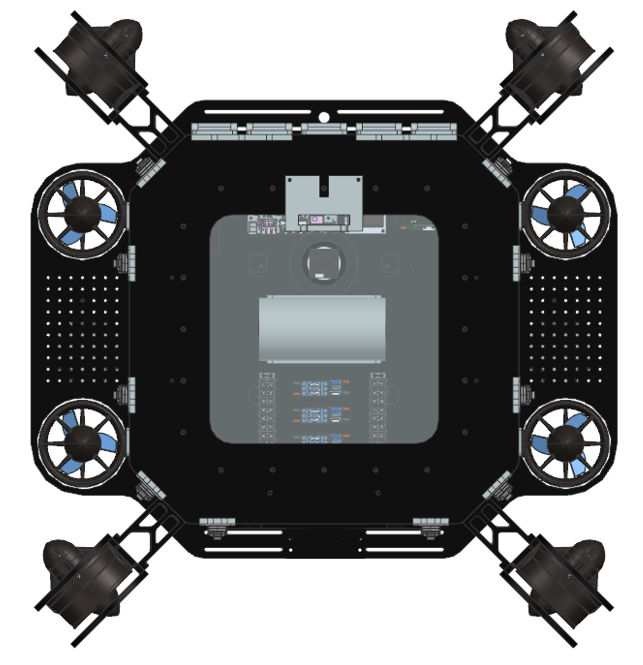
\includegraphics[scale=0.35]{images/FullSub2025Top.png}}
    \caption{CAD of top-view of Theseus.}
    \label{fig:sub3}
\end{figure}

\subsubsection{Hull}

\label{sssec:hull}
Our hull is machined from 6061 aluminum with half inch walls to allow for long term reusability. It is a component we recovered from our previous AUV to reduce manufacturing costs, and its modularity characteristics enable easy modifications. It has three windows, two for a front camera and bottom camera and one that provides visibility to the electrical systems for quick troubleshooting. A double o-ring face seal was used at each port to create a redundant seal that ensures a reliable leak proof sub. A lid is mounted to the hull via hinges and secured in place using latches when the sub is underwater. This hinge and latch system makes accessing electronics a quick and simple process. The submarine also contains an eight-thruster configuration, allowing it to move in all six degrees of freedom (DOF).

To meet the need for frequently shifting components and ballast weights for weight distribution and adding components over time, we included a new bottom plate with a plethora of holes and slots allowing for dynamic redesign. This bottom plate also protects sub’s vertical thrusters from impact. We utilized our modular design to prototype new dropper and grabber mechanisms to the AUV. Slight modifications to the frame around the hull allowed us to add these components while keeping the vehicle slightly positively buoyant.

We also implemented new mounts for the submarine's angled thrusters. These mounts contain thruster shrouds to protect the AUV from wall collisions. We also improved the hydrodynamics of the AUV by redesigning the hull to have reduced thickness, and proportionally reducing the buoyancy foam to achieve near-neutral buoyancy.

\subsubsection{Grabber}
\begin{figure}[h]
    \centerline{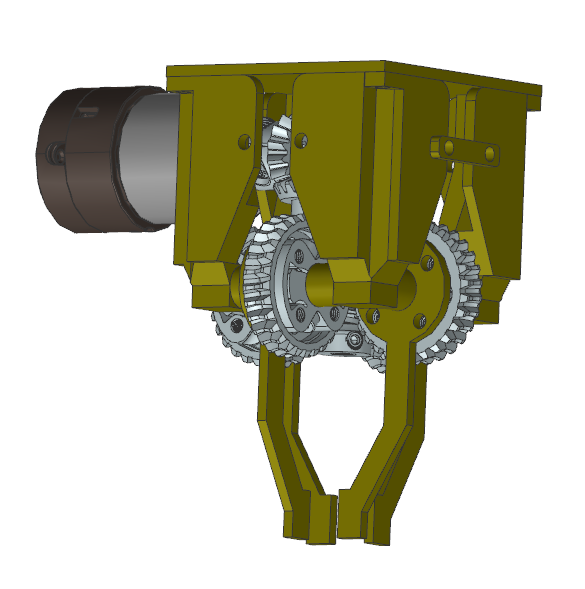
\includegraphics[scale=0.22]{images/CarterGrabberV4.png}}
    \caption{CAD of grabber.}
    \label{fig:grabber}
\end{figure}
\label{sssec:grabber}
To collect and move samples, we implemented a claw mechanism (Fig \ref{fig:grabber}). Our design features four motor-actuated claws linked through a set of worm gears and axles, allowing for a more secure hold on the sample. When the motor spins in one direction, the worm gear spins, causing the claws to move farther apart until a wide enough gap between them opens for them to grab a sample. Meanwhile, clamping onto the sample is a simple matter of reversing the motors to close and secure the sample. The arms and supporting frame were 3-D printed via FDM out of PLA due to their complicated geometries. They are sturdy enough to pick up and hold the samples, while still remaining weaker than the rest of the mechanism, so that they break first in case of a collision, since they are much easier to make and less expensive to replace.



\subsubsection{Dropper}
\label{sssec:dropper}
This year, we also implemented a marker dropper subsystem (Fig \ref{fig:dropper}). In this design, we have chosen to use a single dropper that contains two markers, which can only be dropped one at a time. The dropper is 3-D printed via FDM out of PLA. To hold our markers in place, we have another PLA part that functions as a rotating, T-shaped guide that connects directly to our servo and holds the markers away from the opening on the bottom of our base. 3-D printing was used for the design because it is easy to produce, modify, and replace, and our part does not undergo a lot of stress.

\begin{figure}[h]
    \centerline{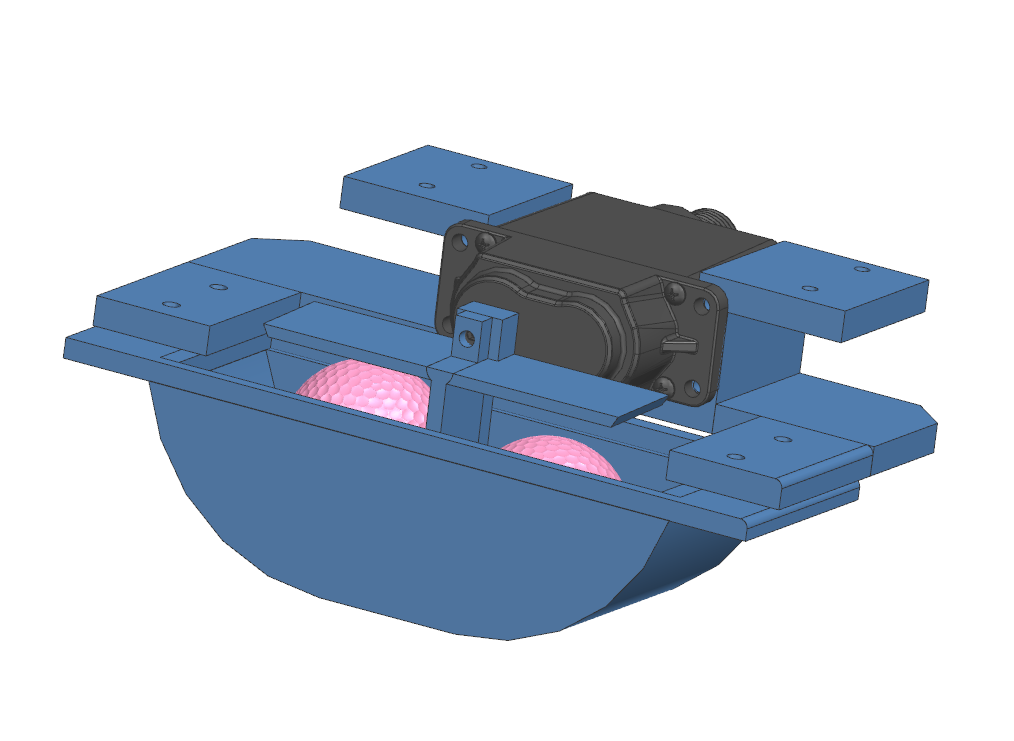
\includegraphics[scale=0.22]{images/Marcus_Dropper.png}}
    \caption{CAD of dropper.}
    \label{fig:dropper}
\end{figure}
\subsubsection{Manufacturing New Submarine}
\label{sssec:New_Sub}
This year, we began manufacturing the new submarine. This new design consists of a 6061 aluminum cylindrical hull that holds our electronics on a sliding tray, connected to a frame of aluminum extrusion. We made the decision to change the shape of our hull from previous years to make all of the manufacturing possible in-house, so we don't have to send out material to get it machined for us, saving money. It has one window on the main hull, for viewing the electronics and for our front camera. Following from our current design, we are using a double o-ring face seal for redundancy and to give us a similar hinge and latch system as before.

Unlike the Montemayor, our new sub does not store the battery in the main hull. Instead, we have a separate acrylic enclosure for it, recovered from our previous AUVs. Doing this will allow us to keep our center of gravity along the midline of the sub, and also keep it low for hydrostatic stability. 

\subsection{Electrical Stack}
\label{ssec:electrical}

\subsubsection{Fuses}
\label{sssec:fuses}
After experiencing an electrical fire while live testing the AUV last year, we decided to implement fuses on multiple components. Accordingly, fuses are integrated on the motor control boards for each ESC, as well as our Doppler Velocity Log (DVL). 

\subsubsection{Hall Effect Sensors}
\label{sssec:hall_effects}
To control the behavior of the AUV while disconnected from its tether, we used two latching hall effect sensors. Magnets trigger these sensors to control the starting, stopping, and resetting of other sensors (in particular, the IMU) without needing a live connection. The ability to quickly control the state of our sensors externally improves the efficiency of our testing setup time. Once a state is activated, an indicator LED is lit for visual verification. 

\subsubsection{Motor Control Board}
\label{sssec:motor_board}
We identified the motor control electrical subsystem as a top priority due to its critical functionality, frequency of maintenance, and large space overhead. Previously, we utilized 4 printed circuit boards (PCB), each containing two electronic speed controllers (ESCs), to control our 8 motors. This became an issue because the circuit boards had a very large footprint, forcing them to be stacked to fit properly inside the submarine. Coupled with the loss of reliable electrical connections after long-term use, maintenance became very difficult. Not only that, the boards relied on an external signal wire for each ESC, meaning that there were 8 wires that individually had to be plugged in.

As a result, we chose to consolidate the 4 PCBs with 2 ESCs each into 2 PCBs of 4 ESCs, halving the number of wires. The ESCs still mount directly to the circuit boards via screw-block terminals for ease of replacement. The boards receive power through an XT60 power connector, which allows for easy and spark-free connections. To reduce the amount of signal wires, each motor board includes an RJ45 port for 4 PWM signal lines. This, tied with a new signal generator board, reduced the number of wires onboard by 14.

\begin{figure}
    \centering
    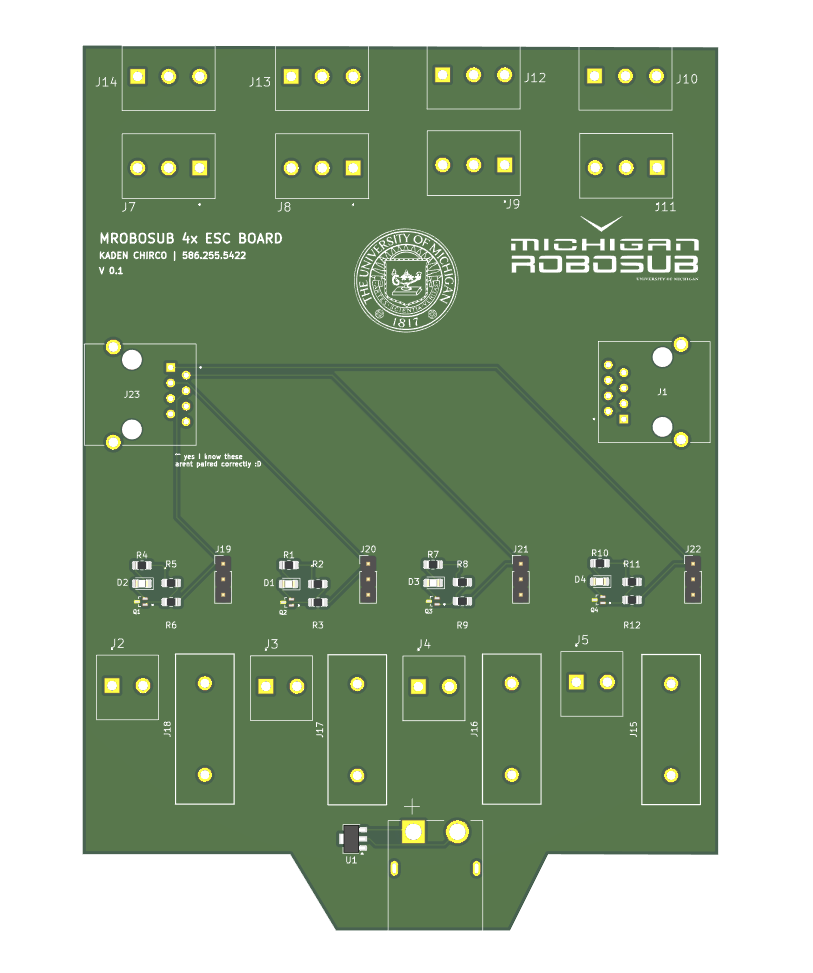
\includegraphics[width=0.5\linewidth]{images/4x ESC Board.png}
    \caption{Motor control board PCB design}
    \label{fig:motor_pcb}
\end{figure}

An important consideration was the current limit for this PCB. The first iteration of this board was operational but failed during prolonged water testing due to insufficient current rating and heat dissipation. The issue was that each ESC could theoretically draw up to 30A which meant the board’s traces had to support this requirement. Increasing the trace width to support 30A was not a good use of space, so we decided to increase the copper weight of each trace, essentially making them ``taller.'' Additionally, we used techniques like dissipating heat with thermal vias and large power and ground planes to fully allow our motor control board to work with multiple ESCs and motors for the second iteration of the board which is currently in use.

\subsubsection{Signal Generator Board}
\label{sssec:signal_board}

While overhauling the motor controlling boards, we also replaced our previous ESC pulse-width modulation (PWM) signal generating board, the Pololu Servo Controller. This was because the device was too complex (leading to technical debt) and suffered intermittent signal loss. As a result, we designed a break-out board for a Xiao ESP32-S3, routing all 8 PWM signals into 2 RJ45 connections. This allowed for a dramatically more organized electrical system while keeping the subsystem as simple as possible for ease of maintenance and future upgrades. 

\begin{figure}
    \centering
    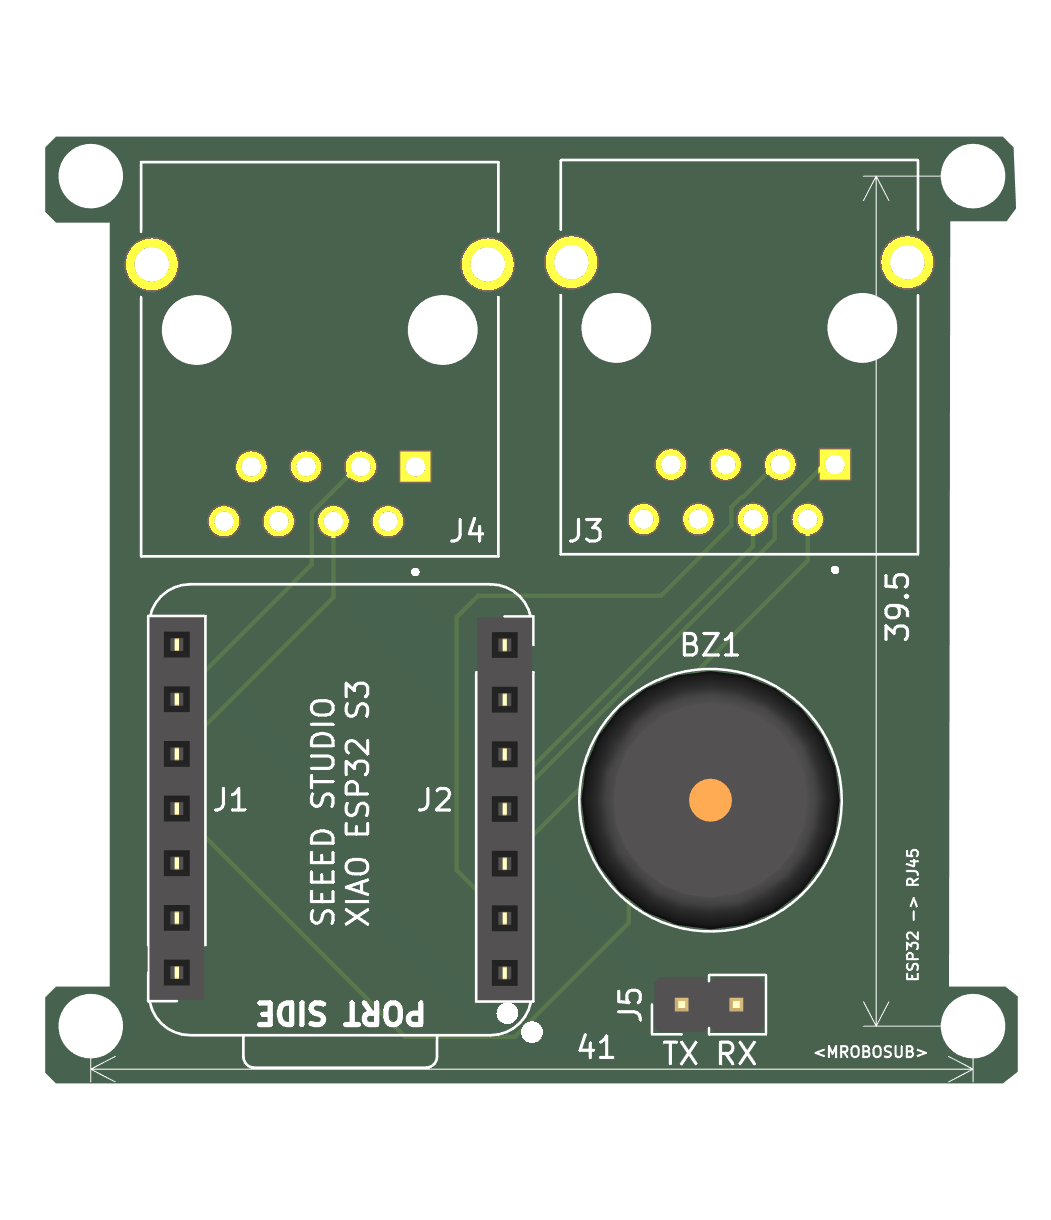
\includegraphics[width=0.5\linewidth]{images/ESP32 Breakout Board.png}
    \caption{Signal generation board PCB design}
    \label{fig:signal_pcb}
\end{figure}

The ESP32 also has the ability to host local networks through a Wi-Fi access point. This was utilized for an online testing suite that can be run on any device. This made testing individual motors much easier than reprogramming an Arduino each time, which was often done in the past.

\subsubsection{Voltage Regulation}
\label{sssec:voltage_regulation}
We continue to use our custom power distribution PCB, which utilizes an off-the-shelf 5V 15A Step Down Regulator as our DC-DC converter to supply up to 75 W to some of our smaller electrical system components. We utilize separate COTS DC-DC converters to supply the Jetson Orin Nano with 12V, tether interface with 7V, and Doppler Velocity Log with 25V.

\subsubsection{Battery Voltage Monitor}
\label{sssec:battery_monitor}
One challenge while operating the submarine has been the need to periodically remove it from the water and measure the battery voltage  to avoid discharging past safe levels. Thus, we designed a custom battery voltage monitor that is visible even once the submarine is sealed. It consists of a custom PCB, an ATTiny85 microcontroller, a TM1637 LED display, and a basic voltage divider circuit.

\subsection{Software Stack}
\label{ssec:software}
Our software stack utilizes ROS2 (Robot Operating System) to distribute our logic into distinct modules called nodes. These nodes are organized into packages based on their role in the AUV's operation. Fig. \ref{fig:software_architecture} shows these packages, with arrows representing the general flow of information between packages. The majority of our code is written in Python, except for some portions of the hardware abstraction layer (HAL), which is written in C++.

\begin{figure}[htbp]
    \centerline{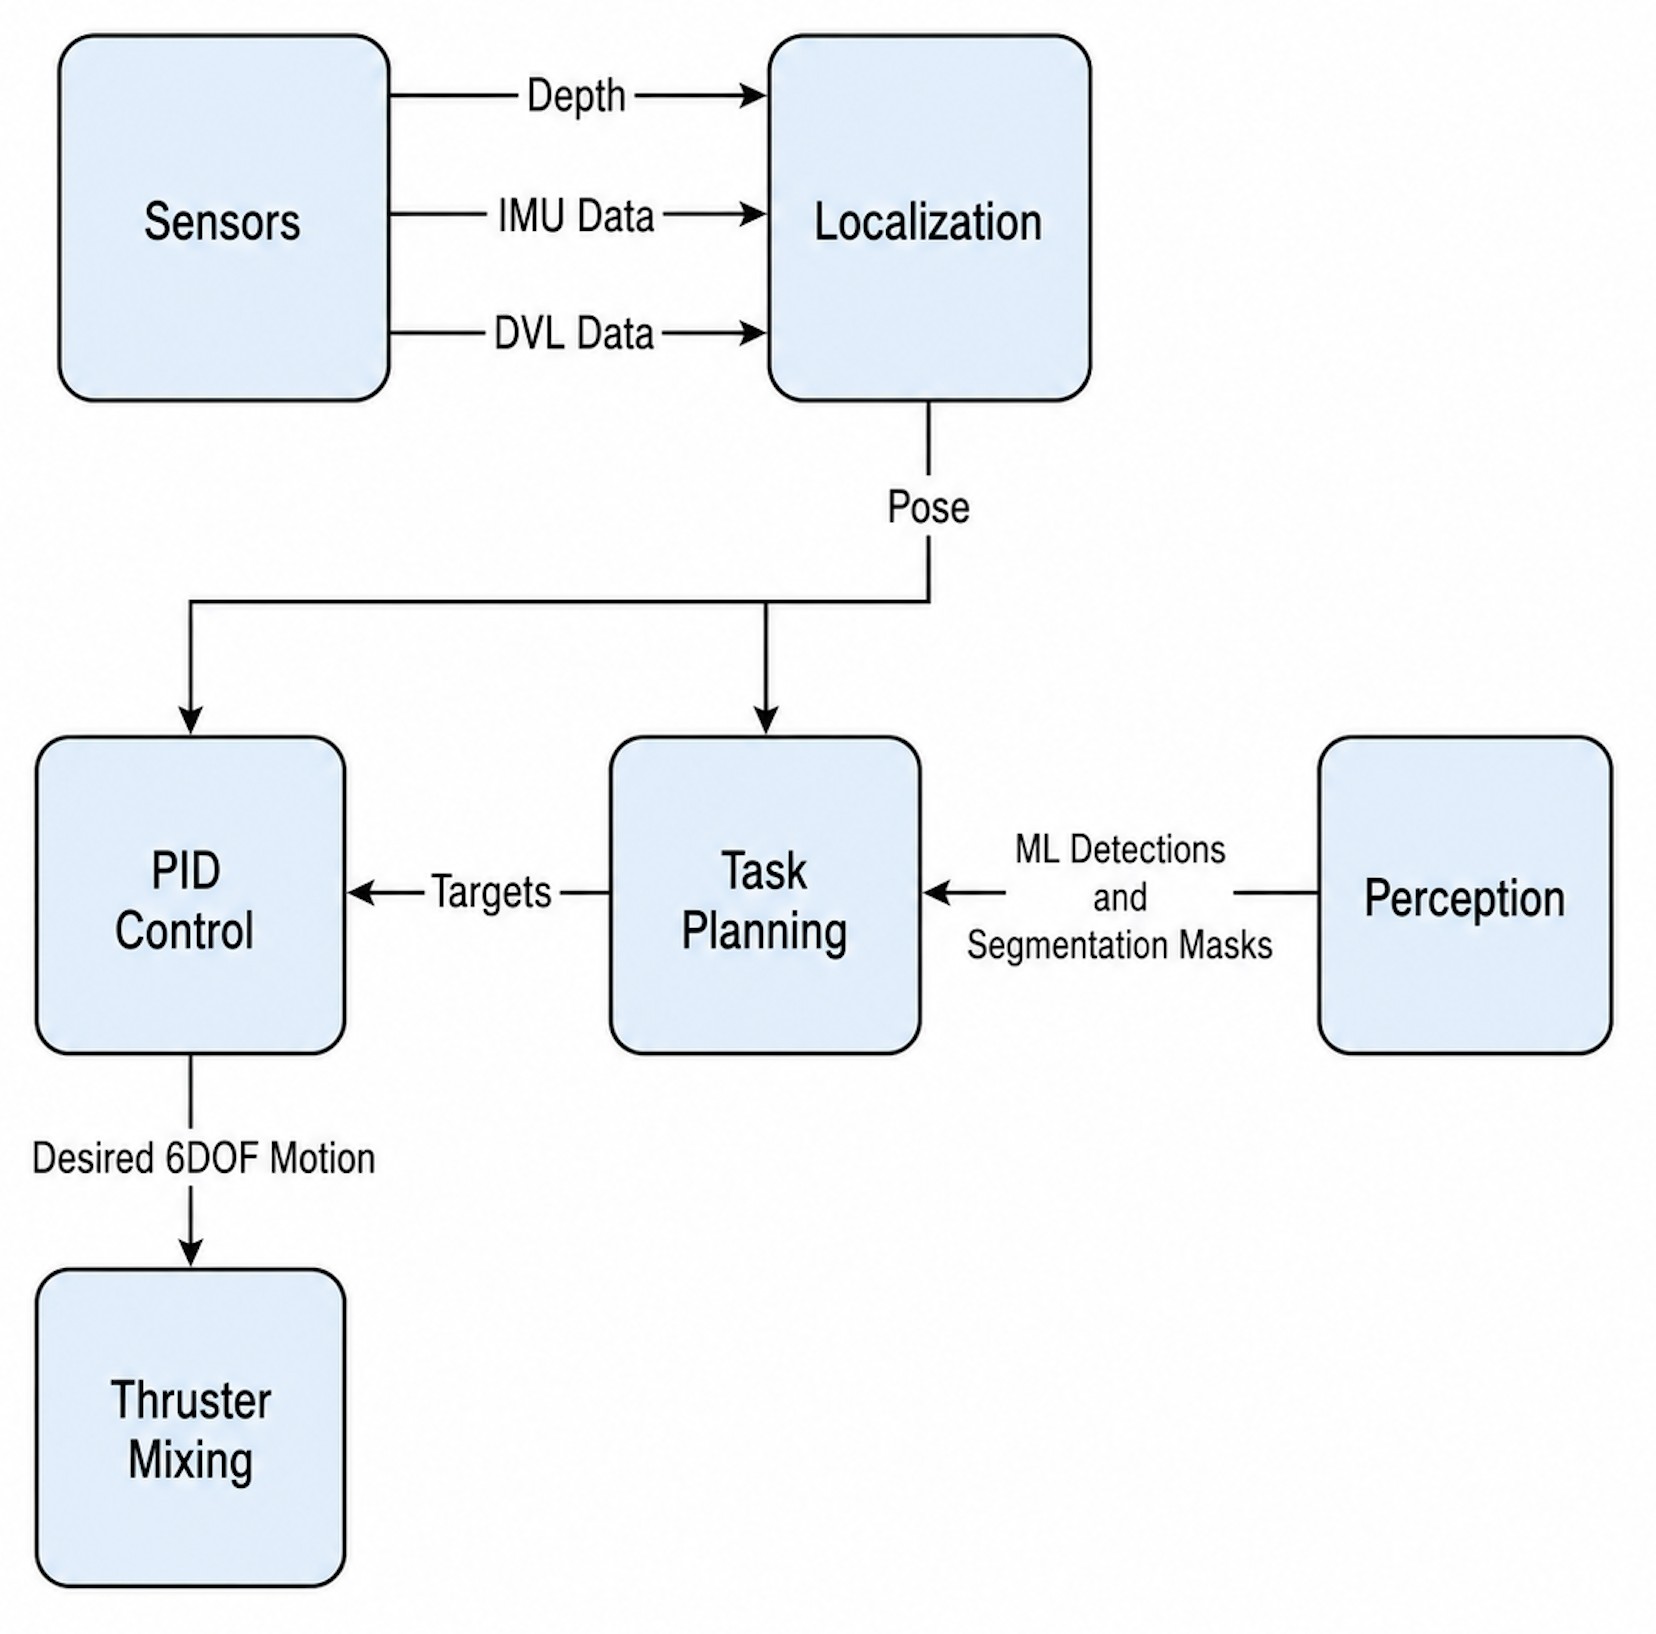
\includegraphics[height=6.5cm, keepaspectratio=false]{images/software_architecture.png}}
    \caption{High-level Software Architecture}
    \label{fig:software_architecture}
\end{figure}

\subsubsection{Computing Architecture}
\label{sssec:comp_arch}
Our computing architecture features a distributed layout to enable greater flexibility and faster iteration. Most of our computing is performed on our Jetson Orin Nano. This is the most powerful computer in the system, so it runs our computer vision, machine learning, high-level planning, localization, and control modules. Among these control modules include our custom thruster control board and driver, and custom thruster mixing code. For interfacing with our low-power devices--namely, our depth sensor, hall-effect sensors, and indicator lights–-we use an Arduino, which the Jetson communicates with via \verb|pyserial|.

\subsubsection{Flight Controller}
\label{sssec:flight_controller}
For the thruster control system, we developed an in-house thruster mixing system and thruster control board driver. Our system was initially designed referencing Tartan AUV's thruster mixing and thruster control code.

The code uses the thruster positions and orientations to construct a non-square matrix that maps the input powers of the eight motors to the vehicle wrench (force/torque in all six DOFs). It then takes the pseudoinverse of this matrix to map desired wrench to motor powers. However, this mapping may request motor powers which exceeding maximum force or current draws, potentially degrading the electrical system of the vehicle. To combat this, the controller dynamically and uniformly scales down the requested input wrench until the computed motor powers fall within predefined power and current limits. The controller then uses a model to determine the input signal to be sent to each motor to produce the desired force, which is a nonlinear function. The relationship between motor input signal, motor output power, and motor current draw (all with respect to system voltage) was calculated by fitting cubic polynomials in the thruster's forward and reverse directions using data provided by the supplier, BlueRobotics \cite{b9}. The polynomial relating PWM motor input and current is shown in Fig. \ref{fig:motor_fits}.

\begin{figure}[htbp]
    \centerline{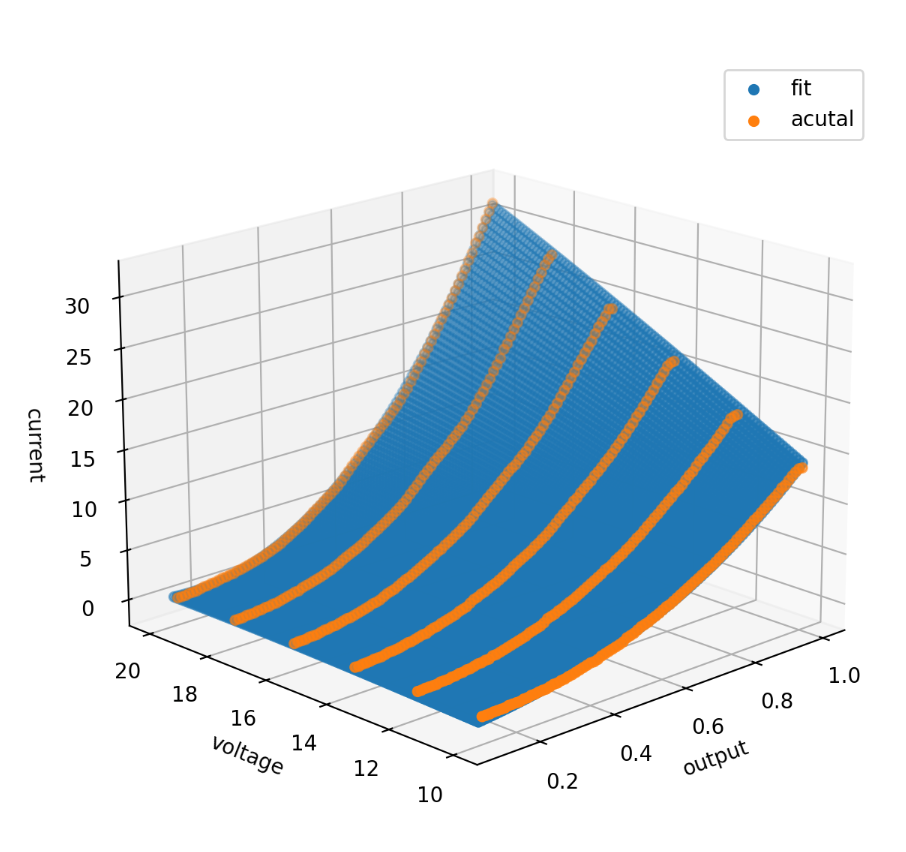
\includegraphics[scale=0.28]{images/motor_fits.png}}
    \caption{Computed motor fit curve relating input voltage, thruster mixing output (i.e., PWM motor input), and current draw.}
    \label{fig:motor_fits}
\end{figure}

\subsubsection{Orientation Sensing}
\label{sssec:orientation_sensing}
% Zayn (05/09/26): We can keep this as-is.
To measure our orientation, we use the InertialSense IK-1-IMX-5 IMU. This IMU was chosen for its high measurement frequency (1 KHz), low rate gyroscopic drift (claimed $0.16^{\circ}/\sqrt{hr}$), and built in Altitude, Heading, and Reference System (AHRS) which fuses measurements from the gyroscope, accelerometer, pressure, and magnetometer sensors into a single accurate orientation estimate. We use the IMU to measure linear acceleration and angular velocity along the x, y, and z axes. We also use the AHRS to provide orientation information to our planning and control algorithms.

%The Inertial Measurement Unit is implemented to measure and report acceleration and angular velocity, and provides general information about AUV orientation and movement. This is vital for the software sub-team to implement thruster mixing and path planning for our AUV.

\subsubsection{Path Marker Detection (Segmentation Model)}
\label{sssec:cv}
% Muskaan is done updating this section as of May 2026
In order to detect the path marker, we historically utilized classical computer vision (CV) techniques based on HSV thresholding. One notable challenge with this approach is the variable lighting conditions faced during the competition depending on the time of day. The bright sunlight, reflecting through the water, caused the AUV to incorrectly consider lines at the bottom of the pool as being within our path marker HSV ranges.

Thus, this year, we have switched using machine learning to detect the path marker. We fine-tune a YOLOv8 segmentation model \cite{b7} on images taken at competition. This model both detects our desired object and gives us a mask for the detection. We then use geometrical methods from OpenCV \cite{b8} to determine the orientation of the path marker from the mask, thus informing our AUV's trajectory.

\subsubsection{Image Detection (YOLOv5 Model)}
\label{sssec:ml_flow}
To detect the images on the gate and in the bins, we continue to use our machine learning pipeline, wherein we fine-tune a YOLOv5 object-detection neural network \cite{b3} using data collected during competition itself. Our model uses the PyTorch framework, an open source machine learning framework that is an industry standard for this type of work \cite{b4}.

We continue to use our 2024 process of labeling data and training models using scripts to automate training on the University of Michigan's Great Lakes Computing high performance compute (HPC) clusters. We created a data pre-processing script to verify image attributes. We then upload images to \href{https://labelbox.com/}{LabelBox} and manually label the dataset. Subsequent scripts generate the label files and segment them into the training and testing designations. To evaluate model performance on unseen data, we utilize a model evaluation script provided by the Ultralytics YOLO package. This allows us to efficiently train our model using only data we collected at the competition itself. This year, we ported our object-detection pipeline to ROS 2, as well as improving robustness and code readability.

\subsubsection{Custom PID}
\label{sssec:custom_pid}
This year, we replaced our third-party PID control library with a custom PID module as the third-party library is not compatible with ROS 2. In our custom control architecture, pose is regulated through six independent PID loops, one for each degree of freedom. We utilize angle wrap-around for rotational DOFs, integral wind-up mitigation via conditional integration and integral clamping, and derivative kick prevention by computing the D-term from delta position rather than delta error.

\subsubsection{Task Planner}
\label{sssec:task_planner}
The task planner is the high-level architect coordinating the interplay of subsystems necessary to complete competition tasks. Our task planner is a state machine, where the AUV is assigned a current state that dictates its logic and may produce a state transition if certain conditions are met.

Transition maps define which new state the vehicle is assigned if a state transition is produced. We use several transition maps to refine various routines, including a complete competition map or specific task maps. We can use different maps at testing time to isolate the relevant behaviors.

In the past few years, we have been significantly improving our state machine framework to reduce operational friction and catch errors before water-test time. These features include state parameter overriding, the ability to start the state machine at any state, and static type checking with \verb|mypy|, allowing our team to more quickly prototype, test, and debug state machine logic. 

\section{Testing Strategy}
\label{sec:testing}

\subsection{Teleoperation Framework}
\label{ssec:teleop}
This year, we entirely re-hauled our teleoperation (teleop) framework, allowing a human driver to manually control the AUV's 6DOF velocities using a Logitech controller, while other subsystems run autonomously. This enables us to gather controlled field data (e.g. for cameras) and debug components in isolation. By writing our own teleop framework, we are not limited to any specific hardware or software such as ArduSub and are able to provide tighter integrations with our other systems. We also mapped specific inputs from the controller to emergency-stop the AUV, as well as to reset sensor and localization readings. Being greatly simplified while maintaining functionality, we have found this teleop framework to be extremely useful for testing and iteration.

\subsection{In-Water Testing}
\label{ssec:in_water_testing}
From past competitions, we have learned that in-water testing is invaluable and allows for both the software and hardware teams to validate their designs. It is also a great opportunity to train new members and boost morale.

This year, we performed our testing at two locations: the U-M Marine Hydrodynamics Laboratory (MHL) towing tank and the U-M Ford Robotics Building (FRB) Tank. These tanks are large enough for us to calibrate sensors and motors, evaluate our control and localization algorithms, and test our state machine's interactions with game elements.

Before each in-water testing session, we prioritized the components that we intended to test. After each session, we reviewed our results and discussed potential system improvements.

\subsection{Off-Board Testing}
\label{ssec:off_board_testing}
To prevent us from wasting in-water testing time on simple software errors, we developed a container image that emulates our main computer to use with virtualization software like Docker and Podman. This allows any team member to write, execute, and test our code on their laptops. In general, we test our software logic within the container and reserve in-water testing system integration and collecting sensor data. We can visualize the state of our vehicle using RViz.

\subsection{Simulation}
\label{ssec:simulation}
To facilitate stronger system integration, debugging, and testing without access to in-water testing, we developed a graphical simulator which communicates bidirectionally with our in-container vehicle software. The architecture of our vehicle software abstracts communication with hardware behind a hardware abstraction layer (HAL); when running on the physical vehicle, the HAL is backed by real sensors and actuators, but when running in simulation, hardware is emulated by virtual devices on a simulated vehicle.

The simulation runs as a game in the Bevy game engine \cite{b10} with Avian physics, chosen because it is easy to build and distribute across all development platforms (Windows, Mac, Linux). The game runs outside the container and communicates sensor/actuator data across TCP sockets. Desired control outputs are aggregated in the vehicle software by a virtual HAL and sent to the simulation. The simulation applies the desired control, and computes expected sensor readings based on the simulated movement of the vehicle. Simulated sensor readings are sent back to the virtual HAL and feed back into higher level control and planning logic.

The simulation incorporates several game elements including the Gate, Slalom, and Bins. Using known camera parameters, the simulation generates predicted object detections, which are used to test higher level planning logic. This helped significantly reduce iteration times because actual machine-learning based object detections are too expensive to run on development machines and access to in-water environments large enough to accommodate multiple game elements was very rare.

\section*{Acknowledgments}
The Michigan Robotic Submarine team would like to thank our 2025-2026 sponsors, listed in Appendix \ref{sec:sponsors}, for their monetary support. We'd also like to thank the individuals who donated to our team during the University of Michigan's Giving Blue Day fundraiser. 

We would also like to thank our advisor Dr. Katie Skinner for continuously supporting our team by advising us and overseeing the Multidisciplinary Design Program, which allows members to earn class credit for their contributions to our team.

We are extremely grateful to the Marine Hydrodynamics Lab staff, especially Jason Bundoff and Nicole Cheesman, for graciously providing the team with an in-water testing location.  We also would like to thank the Wilson Student Team Project Center and Ford Motor Company Robotics Building staff, especially Alyssa Emigh, Chris Gordan, Damen Provost and Daniel Meier, for hosting our team workspace and providing us with a pool testing location.

We also thank Mariah Moss and Katelyn Poore from the Office of Student Affairs at the University of Michigan College of Engineering for their guidance in our team operations and assistance in purchasing components.

We are also grateful for the image data provided through the RoboNation data sharing program. Lastly, we would like to thank the RoboNation team for organizing the RoboSub competition and making all of this possible.

\clearpage
\begin{thebibliography}{00}
\bibitem{b3} G. Jocher, ``ultralytics/yolov5: v6.1 - TensorRT, TensorFlow Edge TPU and OpenVINO Export and Inference''. Zenodo, Feb. 22, 2022. doi: 10.5281/zenodo.6222936.
\bibitem{b4} P. Adam et al., ``PyTorch: An Imperative Style, High-Performance Deep Learning Library,'' in \textit{Advances in Neural Information Processing Systems 32}, Curran Associates, Inc., 2019, pp. 8024--8035.
\bibitem{b5} Inspiration Robotics, ``RoboSub-Simulation''. Github.com. https://github.com/InspirationRobotics/RoboSub-Simulation (accessed June 11, 2022).
\bibitem{b6} S. Macenski, T. Foote, B. Gerkey, C. Lalancette, and W. Woodall, ``Robot Operating System 2: Design, architecture, and uses in the wild,'' \textit{Science Robotics}, vol. 7, no. 66, 2022. doi: 10.1126/scirobotics.abm6074.
\bibitem{b7} G. Jocher, A. Chaurasia, and J. Qiu, ``Ultralytics YOLO,'' 2023. [Online]. Available: https://github.com/ultralytics/ultralytics
\bibitem{b8} G. Bradski, ``The OpenCV Library,'' \textit{Dr. Dobb's Journal of Software Tools}, 2000.
\bibitem{b9} Blue Robotics, ``T200 Thruster Technical Details,'' 2022. [Online]. Available: https://bluerobotics.com/store/thrusters/t100-t200-thrusters/t200-thruster-r2-rp/
\bibitem{b10} Bevy Contributors, ``Bevy: A refreshingly simple data-driven game engine built in Rust,'' 2020. [Online]. Available: https://bevyengine.org

\end{thebibliography}

\vspace{2em}

\appendices

\raggedbottom

\section{Sponsors}
\label{sec:sponsors}

\subsection{Captain}
\label{ssec:captain_sponsors}

\begin{itemize}
    \item University of Michigan College of Engineering
\end{itemize}

\subsection{Commander}
\label{ssec:commander_sponsors}

\begin{itemize}
    \item Ford Motor Company
    \item University of Michigan Robotics Department
    \item University of Michigan Central Student Government
    \item University of Michigan Engineering Student Government
    \item University of Michigan Electrical and Computer Engineering Department
    \item University of Michigan Computer Science and Engineering Department
\end{itemize}

\subsection{Lieutenant}
\label{ssec:lieutenant_sponsors}
\par
\begin{itemize}
    \item University of Michigan Mechanical Engineering Department
    \item ZenBusiness
    \item Adobe
\end{itemize}

\newpage
\clearpage

% \begin{center}
% Zayn (05/09/2026): This can be majorly revamped.
% Colten (05/09/26): Jetson Xavier NX should be Jetson Orin Nano, make sure to replace stats as appropriate

% Muskaan (May 2026):
% add logitech controller remote?


\section{System Components}
\label{sec:system_components}

\begin{table}[htbp] % This will float to the top of the page, appearing beautifully right under the header
\centering
\caption{System Components, Specifications, and Procurement Cost}
\label{table:system_components}
\newcolumntype{Y}{>{\centering\arraybackslash}X}
\renewcommand{\arraystretch}{1.5}
\rowcolors{2}{white}{lightgray}
\begin{tabularx}{\textwidth}{@{} l l Y Y r c @{}}
    \toprule
        \textbf{Component}      & \textbf{Vendor}               & \textbf{Model/Type} & \textbf{Specs}   & \textbf{Cost} & \textbf{Year} \\ 
    %   -------------------------------------------------------------------------------------------------------------------------------------------
        \addlinespace[0.8em]
        \rowcolor{white}\multicolumn{6}{@{}l}{\textbf{Mechanical Subsystems}} \\
        \midrule
        AUV Hull Form           & American Tooling              & Custom              & 6061 aluminum    & \$3,250.00 & 2022             \\ 
        Connectors              & Blue Robotics                 & WetLink Penetrators & WLP-M10 6.5MM-HC & \$120.00   & 2024             \\ 
        Propulsion              & Blue Robotics                 & T200 w/ Propellor   & 7-20V            & \$1,074.00 & 2020             \\ 
        
        \addlinespace[1.5em]
        \rowcolor{white}\multicolumn{6}{@{}l}{\textbf{Electrical \& Sensing Subsystems}} \\
        \midrule
        Power System            & N/A                           & Custom              & Lithium-ion Battery (14.8V, 15.6Ah), 5V and 12V Voltage Regulators, Custom Battery Monitor
      & \textemdash  & 2023          \\ 
        Motor Controls          & Blue Robotics                 & Basic ESC           & 7-26V            & \$172.00   & 2023             \\ 
        CPU & Nvidia & Jetson Orin Nano & 6-core Arm Cortex-A78AE v8.2 @ 1.5 GHz, 8GB LPDDR5 RAM & \$299.00 & 2025 \\ 
        Thruster Board  & N/A                  & Custom    & 2x 4-ESC Boards, XIAO ESP32S3, power/signal connectors & \$7.49 for ESP32  & 2026 \\ 
        IMU  & Inertial Sense       & IK-1-IMX-5          & Accel/Gyro: 10-DOF sensor & \$350.00 & 2025         \\ 
        DVL & Cerulean Sonar             & Tracker 650         & 3 velocity sensors. Max depth: 300m & \$2,990.00 & 2024 \\ 
        Barometer & Blue Robotics & Bar02 Depth Sensor & 0–2 bar (10m depth), I2C, 0.16mm resolution & \$80.00 & 2022 \\
        Camera(s)               & Stereolabs, BR     & ZED2, Low-light HD USB Camera & Stereo vision, pathmarker detection & \$449.00, \$99.00  & 2020, 2021 \\
        Testing Controller & Logitech & Logitech F310 & 10 programmable buttons, 4 switch floating D-Pad & \$19.99 & 2021 \\
        
        \addlinespace[1.5em]
        \rowcolor{white}\multicolumn{6}{@{}l}{\textbf{Software \& Autonomy Architecture}} \\
        \midrule
        Localization & N/A & Custom  & Factor Graph-based sensor fusion & \textemdash & 2026 \\
        Vision                  & N/A                         & YOLOv5 / YOLOv8 & Train CNNs; OpenCV inference  & \textemdash & 2023, 2026\\
        Autonomy                & N/A                          & Custom              & Task-planning state machine   & \textemdash         & 2024\\ 
        GNC & N/A                & Custom              & PID control                   & \textemdash        & 2026 \\ 
        \bottomrule
\end{tabularx}
\end{table}

\end{document}
